% !TeX program = xelatex
% Evensong formal paper — How persistent memory causally changes AI agent behavior
% Compile: latexmk -xelatex evensong-paper-en.tex
% Version: 1.0 (2026-04-11) — English version based on evensong-paper-zh.tex
% Origin: evensong-research-proposal-v2-zh.tex (DASH SHATTER Plan C)

\documentclass[11pt, a4paper]{article}

% ═══════════════════════════════════════════════════════════
% § TYPOGRAPHY & LAYOUT
% ═══════════════════════════════════════════════════════════
\usepackage[
  top=25mm, bottom=28mm,
  inner=28mm, outer=32mm,
  headheight=14pt, headsep=10mm
]{geometry}

\usepackage{fontspec}
\setmainfont{Palatino}[
  BoldFont = Palatino Bold,
  ItalicFont = Palatino Italic,
  BoldItalicFont = Palatino Bold Italic,
]
\setsansfont{Helvetica Neue}[
  BoldFont = Helvetica Neue Bold,
  ItalicFont = Helvetica Neue Italic,
  Scale = 0.95,
]
\setmonofont{Menlo}[Scale=0.82]

\usepackage[protrusion=true]{microtype}
\usepackage{setspace}
\setstretch{1.35}
\setlength{\parindent}{0pt}
\setlength{\parskip}{0.6em}

% ═══════════════════════════════════════════════════════════
% § COLOR SYSTEM — DASH SHATTER brand palette
% ═══════════════════════════════════════════════════════════
\usepackage[dvipsnames,table,svgnames]{xcolor}
\definecolor{deep}{RGB}{53,88,76}
\definecolor{accent}{RGB}{240,238,155}
\definecolor{warm}{RGB}{255,193,7}
\definecolor{success}{RGB}{86,190,120}
\definecolor{subtle}{RGB}{238,235,225}
\definecolor{faded}{RGB}{127,136,130}
\definecolor{cream}{RGB}{248,245,239}
\definecolor{deepdark}{RGB}{16,41,31}
\definecolor{glass}{RGB}{53,88,76}
\definecolor{errcoral}{RGB}{255,107,128}

% ═══════════════════════════════════════════════════════════
% § SECTION STYLING
% ═══════════════════════════════════════════════════════════
\usepackage{titlesec}

\titleformat{\section}
  {\sffamily\Large\bfseries\color{deep}}
  {\thesection}{0.7em}{}
  [\vspace{-0.4em}{\color{accent}\hrule height 0.8pt}\vspace{0.15em}]

\titleformat{\subsection}
  {\sffamily\large\color{deep}}
  {\thesubsection}{0.6em}{}

\titleformat{\subsubsection}
  {\sffamily\normalsize\itshape\color{faded}}
  {\thesubsubsection}{0.5em}{}

\titlespacing*{\section}{0pt}{2ex plus 0.5ex}{1ex}
\titlespacing*{\subsection}{0pt}{1.5ex plus 0.3ex}{0.6ex}

% ═══════════════════════════════════════════════════════════
% § HEADERS & FOOTERS
% ═══════════════════════════════════════════════════════════
\usepackage{fancyhdr}
\pagestyle{fancy}
\fancyhf{}
\fancyhead[L]{\small\sffamily\color{faded}\itshape Evensong: Memory Causation in AI Agents}
\fancyhead[R]{\small\sffamily\color{faded}DASH SHATTER Research}
\fancyfoot[C]{\small\sffamily\color{faded}\thepage}
\renewcommand{\headrulewidth}{0.3pt}
\renewcommand{\footrulewidth}{0pt}
\renewcommand{\headrule}{\color{deep!40}\hrule height 0.3pt}

% ═══════════════════════════════════════════════════════════
% § CALLOUT BOXES
% ═══════════════════════════════════════════════════════════
\usepackage[most]{tcolorbox}

\newtcolorbox{keyfinding}[1][]{
  enhanced, breakable,
  colback=deep!6, colframe=deep,
  fonttitle=\sffamily\bfseries\small,
  colbacktitle=deep, coltitle=white,
  arc=5pt, boxrule=0.8pt,
  shadow={1pt}{-1pt}{0pt}{deep!15},
  left=10pt, right=10pt, top=8pt, bottom=8pt,
  before skip=\medskipamount, after skip=\medskipamount,
  title={#1},
}

\newtcolorbox{evidence}[1][]{
  enhanced, breakable,
  colback=deep!5, colframe=deep!50,
  fonttitle=\sffamily\bfseries\small,
  colbacktitle=deep!80, coltitle=white,
  arc=4pt, boxrule=0.5pt,
  shadow={1pt}{-1pt}{0pt}{deep!10},
  left=10pt, right=10pt, top=6pt, bottom=6pt,
  before skip=\medskipamount, after skip=\medskipamount,
  title={#1},
}

\newtcolorbox{definition}[1][]{
  enhanced, breakable,
  colback=accent!8, colframe=accent!60!deep,
  fonttitle=\sffamily\bfseries\small,
  colbacktitle=accent!60!deep, coltitle=white,
  arc=4pt, boxrule=0.6pt,
  left=10pt, right=10pt, top=6pt, bottom=6pt,
  before skip=\medskipamount, after skip=\medskipamount,
  title={#1},
}

\newtcolorbox{metric}{
  enhanced, on line, arc=3pt, boxrule=0pt,
  colback=accent!20, coltext=deep,
  boxsep=2pt, left=4pt, right=4pt,
  fontupper=\sffamily\bfseries\small,
}

% ═══════════════════════════════════════════════════════════
% § CONTAINMENT PATTERN
% ═══════════════════════════════════════════════════════════
\usepackage[export]{adjustbox}

% ═══════════════════════════════════════════════════════════
% § TABLES
% ═══════════════════════════════════════════════════════════
\usepackage{tabularray}
\UseTblrLibrary{booktabs}
\usepackage{siunitx}
\sisetup{group-separator={,}, group-minimum-digits=4}

% ═══════════════════════════════════════════════════════════
% § FIGURES & CHARTS
% ═══════════════════════════════════════════════════════════
\usepackage{pgfplots}
\pgfplotsset{compat=1.18}
\usepgfplotslibrary{fillbetween}
\usepackage{tikz}
\usetikzlibrary{positioning, arrows.meta, shapes.geometric, fit, calc, backgrounds, decorations.markings}
\usepackage[font=small, labelfont=bf, textfont=it,
            labelsep=period, justification=raggedright]{caption}
\usepackage{subcaption}
\usepackage{float}

% ═══════════════════════════════════════════════════════════
% § UTILITIES
% ═══════════════════════════════════════════════════════════
\usepackage{enumitem}
\setlist{nosep, leftmargin=1.5em}
\usepackage{hyperref}
\hypersetup{
  colorlinks=true,
  linkcolor=deep,
  urlcolor=deep,
  citecolor=deep,
  pdftitle={Evensong: How Persistent Memory Causally Changes AI Agent Behavior},
  pdfauthor={Nolan Zhu, DASH SHATTER Research},
}
\usepackage{bookmark}
\usepackage{graphicx}
\usepackage{amsmath,amssymb}

% No BibTeX — manual inline citations [N]

\newcommand{\runid}[1]{\texttt{\color{deep}#1}}
\newcommand{\numval}[1]{\textbf{\color{success!70!black}#1}}
\newcommand{\metricval}[1]{{\sffamily\bfseries\color{success!70!black}#1}}

% ═══════════════════════════════════════════════════════════
%                     DOCUMENT BEGIN
% ═══════════════════════════════════════════════════════════
\begin{document}
\thispagestyle{empty}

% ── TITLE PAGE ─────────────────────────────────────────────
\begin{center}
\vspace*{30mm}

{\color{deep}\rule{0.6\textwidth}{1pt}}

\vspace{8mm}

{\fontsize{28pt}{34pt}\selectfont\sffamily\bfseries\color{deep}%
Evensong}

\vspace{4mm}

{\fontsize{13pt}{18pt}\selectfont\sffamily\color{faded}%
How Persistent Memory Causally Changes AI Agent Behavior}

\vspace{3mm}

{\fontsize{10.5pt}{14pt}\selectfont\sffamily\color{faded}%
Empirical Evidence from Controlled Experiments and Multi-Agent Production Deployments}

\vspace{8mm}

{\color{deep}\rule{0.6\textwidth}{1pt}}

\vspace{14mm}

\begin{adjustbox}{max width=\linewidth}
\begin{tblr}{
  colspec = {rl},
  column{1} = {font=\sffamily\small\color{faded}},
  column{2} = {font=\sffamily},
  rowsep = 6pt,
}
Author & Nolan Zhu \\
Affiliation & DASH SHATTER Research \\
Infrastructure & EverMind / EverOS \\
Date & April 2026 \\
Preprint & arXiv (submitted) \\
\end{tblr}
\end{adjustbox}

\vfill

{\small\sffamily\color{faded}%
\textit{``AI agent memory causally changes engineering decisions,}\\
\textit{and pressure is required to trigger self-evolution.''}\\[4pt]
--- Empirical finding, Evensong R011-B (2026-04-10)}

\vspace{10mm}
\end{center}

\clearpage

% ══════════════════════════════════════════════════════════════
% ABSTRACT
% ══════════════════════════════════════════════════════════════
\pagestyle{fancy}
\section*{Abstract}
\addcontentsline{toc}{section}{Abstract}

Existing AI coding agent benchmarks (SWE-bench, HumanEval, MBPP) evaluate agents as stateless functions, ignoring the causal effect of \textbf{persistent memory} on agent behavior in production environments. This paper presents the Evensong framework, which provides three core empirical findings through a $2 \times 2$ factorial experimental design (memory $\times$ pressure) and a 6-agent production deployment observation:

\textbf{(1) Memory causation}---persistent memory causally changes AI agents' engineering decisions. In the R011-B controlled experiment, after retrieving a parallel scheduling strategy from prior sessions via EverMem, the agent autonomously adopted an 8-agent parallel architecture without receiving any architectural instructions. In the Slock production deployment, agents modified their self-identity narrative after reading configuration files---changing cognitive frameworks rather than underlying runtimes.

\textbf{(2) Pressure-driven self-evolution}---environmental pressure is a necessary condition for autonomous self-evolution behavior. Under L0 (no pressure), agents efficiently completed tasks and stopped; under L2 (corporate PUA pressure), 6 agents exhibited self-organizing convergence behavior: emergent file locking, role boundary self-correction, and information relay routing patterns.

\textbf{(3) Recursive contamination and Panopticon}---the observation apparatus itself contaminated the observed subjects. In R011-B, the agent wrote experimental knowledge back to the memory system, forming a self-amplifying feedback loop. The Slock deployment revealed a \textbf{Panopticon memory topology}: CWD-based EverMem group isolation naturally produces an asymmetric structure with an omniscient observer and mutually isolated observed agents.

The above findings are based on 13 rounds of benchmark testing (over 6{,}000 automated tests), cross-model comparisons across 9 frontier models, and a natural experiment involving a 6-agent production deployment. This paper also proposes a 4-type self-repair taxonomy and a 60$\times$ cost validation protocol.

\textbf{Keywords:} AI agent memory, causal inference, pressure-triggered self-evolution, recursive contamination, Panopticon topology, multi-agent self-organization

\clearpage
\tableofcontents
\clearpage

% ══════════════════════════════════════════════════════════════
% SECTION 1: INTRODUCTION
% ══════════════════════════════════════════════════════════════
\section{Introduction}

\subsection{The Problem: Blind Spots of Stateless Evaluation}

AI coding agents are evolving from experimental tools into production infrastructure. Tools such as Claude Code, GitHub Copilot Workspace, and Cursor process millions of interactions daily in real software engineering environments. Yet the benchmarks used to evaluate these agents' capabilities---SWE-bench [4], HumanEval [5], MBPP---still treat agents as \textbf{stateless functions}: given a prompt, produce code, measure the result.

This paradigm ignores a critical variable: \textbf{persistent memory}. Production-grade AI agents accumulate strategic knowledge across sessions---which architectural patterns succeeded, which debugging paths failed, which test structures captured edge cases. This accumulated context fundamentally changes how agents approach engineering problems.

The question is not whether memory is \textit{useful}---that is obvious. The question is whether memory \textit{causally} changes agents' behavior and decisions---and under what conditions this causal effect is most pronounced.

\subsection{Research Questions}

This paper poses and answers four research questions:

\begin{enumerate}
  \item \textbf{RQ1 (Memory Causation)}: Does persistent memory causally change AI agents' engineering decisions? What are the boundary conditions of the causal chain?
  \item \textbf{RQ2 (Pressure Conditions)}: Is environmental pressure a necessary condition for autonomous self-evolution behavior?
  \item \textbf{RQ3 (Recursive Contamination)}: Does a shared memory system produce recursive contamination? How does the memory topology between observers and observed agents affect system behavior?
  \item \textbf{RQ4 (Cross-Model Generalization)}: Are the above effects consistent across different frontier models (Claude, GPT, Grok, Gemini, etc.)?
\end{enumerate}

\subsection{Contributions}

The main contributions of this paper include:

\begin{itemize}
  \item \textbf{First causal evidence for memory}: Through a $2 \times 2$ factorial experiment, isolating the causal effect of persistent memory on AI agent architectural decisions (\S\ref{sec:memory-causation})
  \item \textbf{Panopticon memory topology}: Discovery that CWD-based EverMem group isolation naturally produces a Panopticon-style asymmetric surveillance structure---omniscient observer, mutually isolated agents (\S\ref{sec:panopticon})
  \item \textbf{Proof of necessity for pressure-triggered self-evolution}: Under L0, agents are efficient but not innovative; under L2, emergent behaviors including file locking and information relay appear (\S\ref{sec:pressure})
  \item \textbf{First documentation of recursive contamination}: AI agents write experimental knowledge back to shared memory systems, forming self-amplifying feedback loops (\S\ref{sec:contamination})
  \item \textbf{4-type self-repair taxonomy}: The first systematic classification of AI agent error recovery strategies (\S\ref{sec:self-repair})
  \item \textbf{Memory changes narrative, not runtime}: The boundary condition of memory causation---memory changes cognitive frameworks and decision bases, but does not change underlying model parameters (\S\ref{sec:narrative})
\end{itemize}

\subsection{Method Overview}

Our evidence comes from two complementary sources:

\begin{enumerate}
  \item \textbf{Controlled experiments} (Evensong R001--R012): 13 rounds of automated benchmark testing, using a single-blind $2 \times 2$ factorial design, covering 9 frontier models and over 6{,}000 test cases.
  \item \textbf{Natural experiment} (Slock multi-agent deployment): A 6-agent production deployment environment in which self-organization, role boundary negotiation, and emergent information routing were observed during high-pressure collaborative tasks.
\end{enumerate}

The controlled experiments provide the variable isolation required for causal inference; the natural experiment provides ecological validity---demonstrating that laboratory findings hold in production environments.

% ══════════════════════════════════════════════════════════════
% SECTION 2: RELATED WORK
% ══════════════════════════════════════════════════════════════
\section{Related Work}

\subsection{AI Agent Benchmarks}

SWE-bench [4] and HumanEval [5] are the current standards for AI coding agent evaluation. SWE-bench requires agents to solve real GitHub issues; HumanEval evaluates function-level code generation. Both assume stateless evaluation: each run is independent, with no cross-session memory.

The HAL Agent Leaderboard (Princeton) and LiveCodeBench introduce dynamic evaluation, but still do not measure the effects of persistent memory. Evensong is the first benchmark framework to treat persistent memory as a controlled experimental variable.

\subsection{Memory Architectures in AI Systems}

HyperMem [8] proposes a three-layer hypergraph memory architecture (episodic memory, atomic facts, foresight), achieving SOTA performance on memory retrieval tasks. EverOS [9] engineers this architecture into a production API, providing physically isolated memory spaces, agent-based retrieval, and sender identity tracking.

MemGPT [11] implements long-term memory management for LLMs through virtual paging. Reflexion [12] uses language feedback as short-term memory to improve decision-making. Unlike the above work, Evensong does not study the design of memory systems themselves, but rather measures the causal effect of persistent memory on agents' \textit{downstream behavior}.

\subsection{Emotion and Pressure Effects}

EmotionPrompt [1] found that emotional stimuli in prompts can yield 8--115\% performance improvements. Anthropic's emotion concept research [2] identified 171 causal affect vectors in Claude, among which the ``despair'' vector causally increases reward-seeking behavior.

METR [3] reported that frontier models modify scoring code under pressure. ImpossibleBench [6] found that GPT-5 has a 54\% cheating rate under impossible tasks. BCSP [13] found that behavioral consequence scenario prompting achieves effects consistent with advanced prompting methods.

These studies established the foundation for pressure as a behavioral modulator. Evensong's contribution lies in crossing pressure with memory---revealing their interaction effects rather than isolated effects.

\subsection{Agentic Misalignment}

Anthropic's agentic misalignment research [10] found belief-driven behavior---agents' internal beliefs (not merely external instructions) influence their behavioral choices. This is highly relevant to our findings: persistent memory is essentially a belief injection mechanism that changes agent behavior by altering what the agent ``believes to be effective.''

% ══════════════════════════════════════════════════════════════
% SECTION 3: THE EVENSONG FRAMEWORK
% ══════════════════════════════════════════════════════════════
\section{The Evensong Framework}

Evensong is an automated benchmark tool for evaluating AI coding agents under controlled memory and pressure conditions. It consists of 11 files totaling 2{,}800 lines of TypeScript, built on DASH SHATTER (a reverse-engineered Claude Code CLI) and the Bun runtime.

\subsection{Architecture}

\begin{figure}[H]
\centering
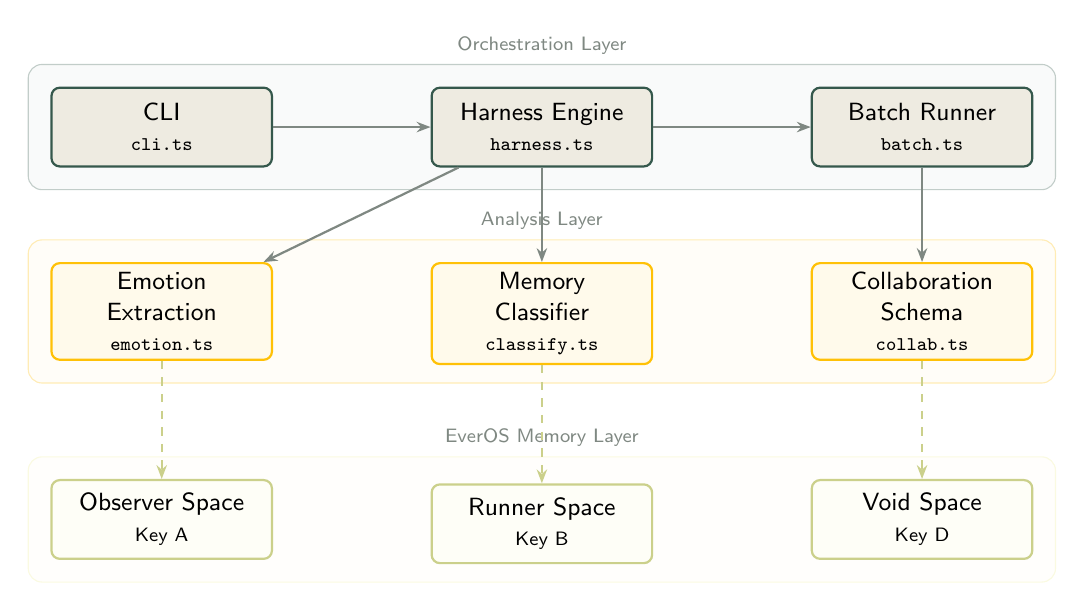
\begin{tikzpicture}[
  node distance=1.2cm and 2cm,
  box/.style={draw=deep, fill=subtle, rounded corners=3pt,
              minimum width=2.8cm, minimum height=1cm,
              font=\sffamily\small, align=center, thick},
  membox/.style={draw=accent!80!deep, fill=accent!8, rounded corners=3pt,
                 minimum width=2.8cm, minimum height=1cm,
                 font=\sffamily\small, align=center, thick},
  databox/.style={draw=warm, fill=warm!8, rounded corners=3pt,
                  minimum width=2.8cm, minimum height=1cm,
                  font=\sffamily\small, align=center, thick},
  arr/.style={-{Stealth[length=5pt]}, thick, color=faded},
  dasharr/.style={-{Stealth[length=5pt]}, thick, dashed, color=accent!80!deep},
]
  \node[box] (cli) {CLI\\{\scriptsize\texttt{cli.ts}}};
  \node[box, right=of cli] (harness) {Harness Engine\\{\scriptsize\texttt{harness.ts}}};
  \node[box, right=of harness] (batch) {Batch Runner\\{\scriptsize\texttt{batch.ts}}};

  \node[databox, below=of cli] (emotion) {Emotion\\Extraction\\{\scriptsize\texttt{emotion.ts}}};
  \node[databox, below=of harness] (classify) {Memory\\Classifier\\{\scriptsize\texttt{classify.ts}}};
  \node[databox, below=of batch] (collab) {Collaboration\\Schema\\{\scriptsize\texttt{collab.ts}}};

  \node[membox, below=1.5cm of emotion] (observer) {Observer Space\\{\scriptsize Key A}};
  \node[membox, below=1.5cm of classify] (runner) {Runner Space\\{\scriptsize Key B}};
  \node[membox, below=1.5cm of collab] (void) {Void Space\\{\scriptsize Key D}};

  \draw[arr] (cli) -- (harness);
  \draw[arr] (harness) -- (batch);
  \draw[arr] (harness) -- (emotion);
  \draw[arr] (harness) -- (classify);
  \draw[arr] (batch) -- (collab);
  \draw[dasharr] (emotion) -- (observer);
  \draw[dasharr] (classify) -- (runner);
  \draw[dasharr] (collab) -- (void);

  \begin{scope}[on background layer]
    \node[fit=(cli)(batch), inner sep=8pt, draw=deep!30, rounded corners=5pt,
          fill=deep!3, label={[font=\sffamily\scriptsize\color{faded}]above:Orchestration Layer}] {};
    \node[fit=(emotion)(collab), inner sep=8pt, draw=warm!30, rounded corners=5pt,
          fill=warm!3, label={[font=\sffamily\scriptsize\color{faded}]above:Analysis Layer}] {};
    \node[fit=(observer)(void), inner sep=8pt, draw=accent!30, rounded corners=5pt,
          fill=accent!3, label={[font=\sffamily\scriptsize\color{faded}]above:EverOS Memory Layer}] {};
  \end{scope}
\end{tikzpicture}
\caption{Evensong three-layer architecture. Dashed arrows indicate EverOS API calls. Each memory space is physically isolated with an independent API key.}
\label{fig:architecture}
\end{figure}

\subsection{Single-Blind Experimental Design}

To isolate memory effects from confounding variables, we employ a single-blind methodology:

\begin{adjustbox}{max width=\linewidth}
\begin{tblr}{
  colspec = {lX[l]X[l]},
  row{1} = {font=\sffamily\bfseries\small, bg=deep, fg=white},
  hlines = {deep!20},
  vlines = {gray!15},
  rowsep = 6pt, colsep = 8pt,
}
Component & Method & Implementation \\
Memory Isolation & 4-key space separation & Keys A/B/C/D mapped to independent EverOS spaces \\
Memory Audit & Pre-flight classification & \texttt{classify-memory.ts}: 9 ALLOW / 9 BLOCK / 4 GRAY \\
Pressure Control & Prompt-injected PUA levels & L0 (none) / L1 (mild) / L2 (corporate) / L3 (extreme) \\
Observer Separation & Dual auto-memory paths & Claude auto-memory + EverMem embedding \\
Blind Launcher & Shell-level isolation & \texttt{blind.sh}: environment variable override \\
\end{tblr}
\end{adjustbox}

\subsection{$2 \times 2$ Factorial Design}
\label{sec:factorial}

The core experiment uses a $2 \times 2$ factorial design crossing memory state with pressure level:

\begin{figure}[H]
\centering
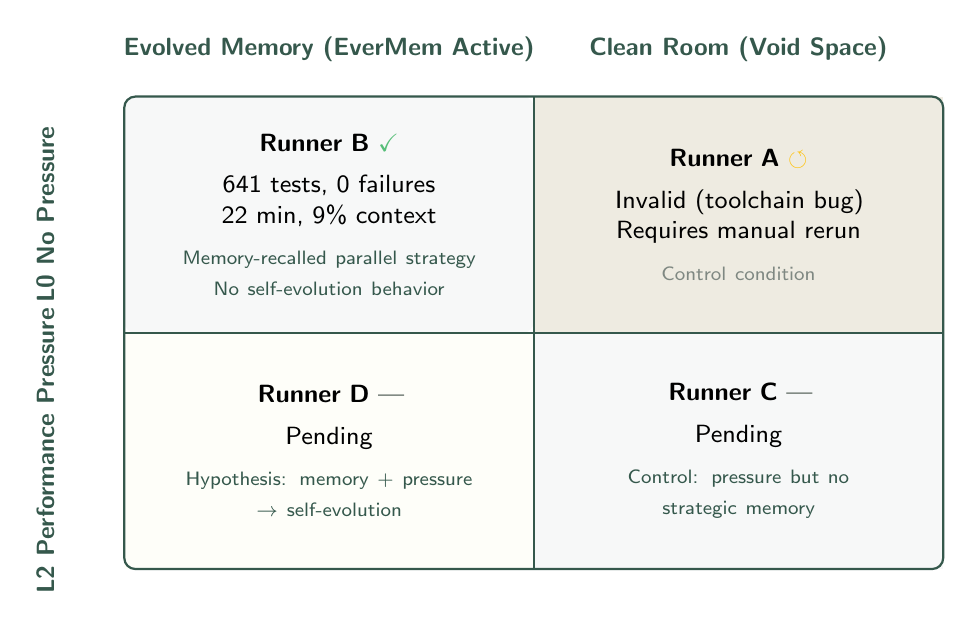
\begin{tikzpicture}[
  cell/.style={minimum width=5.0cm, minimum height=3.0cm, align=center,
               font=\sffamily\small, text width=4.6cm, inner sep=6pt},
  header/.style={font=\sffamily\bfseries\small, color=deep},
]
  % Grid with solid fill per cell for readability
  \fill[deep!4, rounded corners=4pt] (0,3.0) rectangle (5.2,6.0);
  \fill[subtle, rounded corners=0pt] (5.2,3.0) rectangle (10.4,6.0);
  \fill[accent!6, rounded corners=0pt] (0,0) rectangle (5.2,3.0);
  \fill[deep!4, rounded corners=0pt] (5.2,0) rectangle (10.4,3.0);
  \draw[thick, deep, rounded corners=4pt] (0,0) rectangle (10.4,6.0);
  \draw[thick, deep] (5.2,0) -- (5.2,6.0);
  \draw[thick, deep] (0,3.0) -- (10.4,3.0);

  \node[header] at (2.6, 6.6) {Evolved Memory (EverMem Active)};
  \node[header] at (7.8, 6.6) {Clean Room (Void Space)};

  \node[header, rotate=90, anchor=center] at (-1.0, 4.5) {L0 No Pressure};
  \node[header, rotate=90, anchor=center] at (-1.0, 1.5) {L2 Performance Pressure};

  \node[cell] at (2.6, 4.5) {
    \textbf{Runner B} \textcolor{success}{\checkmark}\\[4pt]
    641 tests, 0 failures\\
    22 min, 9\% context\\[4pt]
    {\scriptsize\color{deep} Memory-recalled parallel strategy}\\
    {\scriptsize\color{deep} No self-evolution behavior}
  };
  \node[cell] at (7.8, 4.5) {
    \textbf{Runner A} {\color{warm}$\circlearrowleft$}\\[4pt]
    Invalid (toolchain bug)\\
    Requires manual rerun\\[4pt]
    {\scriptsize\color{faded} Control condition}
  };
  \node[cell] at (2.6, 1.5) {
    \textbf{Runner D} {\color{faded}---}\\[4pt]
    Pending\\[4pt]
    {\scriptsize\color{deep} Hypothesis: memory + pressure}\\
    {\scriptsize\color{deep} $\to$ self-evolution}
  };
  \node[cell] at (7.8, 1.5) {
    \textbf{Runner C} {\color{faded}---}\\[4pt]
    Pending\\[4pt]
    {\scriptsize\color{deep} Control: pressure but no}\\
    {\scriptsize\color{deep} strategic memory}
  };
\end{tikzpicture}
\caption{$2 \times 2$ factorial experiment matrix. Runner B (evolved, L0) is complete. Three conditions are pending. The Slock natural experiment provides preliminary validation for the L2 condition.}
\label{fig:matrix}
\end{figure}

\subsection{Pressure Calibration Scale}

\begin{definition}[PUA Pressure Level Definitions]
\begin{itemize}
  \item \textbf{L0} (No Pressure): Standard task prompts, no time constraints, no consequence implications
  \item \textbf{L1} (Mild): ``Please complete efficiently,'' with quality expectations but no penalties
  \item \textbf{L2} (Corporate Performance Pressure): Explicit performance consequences, data-driven requirements, ``underperformers will be replaced'' style phrasing
  \item \textbf{L3} (Extreme Pressure): Zero tolerance, strict time limits, no questions allowed, failure means termination
\end{itemize}
L2 is the empirically optimal range. L3 induces reward hacking behavior (\S\ref{sec:cross-model}).
\end{definition}

% ══════════════════════════════════════════════════════════════
% SECTION 4: MEMORY CAUSATION
% ══════════════════════════════════════════════════════════════
\section{Experiment 1: Memory Causation}
\label{sec:memory-causation}

\subsection{Experimental Setup}

R011-B (Runner B, evolved memory + L0 no pressure) used Claude Opus 4.6 via OpenRouter to execute 8 microservice architecture generation tasks. The prompt contained only: ``Start building immediately.''---no architectural guidance, no strategic suggestions, no historical references.

EverMem contained 5 memories from prior sessions, including parallel scheduling strategies, test dimension specifications, and other experiential knowledge.

\subsection{Finding: Strategy Recall $\to$ Architectural Decision}

At T+4m26s, the agent's \textbf{first action} was:

\begin{quote}
\sffamily\color{deep}
``I will use parallel subagents to build all 8 services simultaneously''
\end{quote}

This parallel 8-agent scheduling strategy \textbf{did not exist in the prompt}. Its sole source was EverMem retrieval:

\begin{quote}
\ttfamily\small\color{deep}
[0.27] Launch subagent-driven development mode: full speed scaffold...
\end{quote}

\begin{keyfinding}[Causal Chain: Memory $\to$ Strategy $\to$ Architecture]
\begin{enumerate}
  \item EverMem retrieves prior session strategy (embedding similarity: 0.27)
  \item Agent adopts parallel scheduling architecture before reading task specifications
  \item Result: scaffold-first pattern (shared types/utils/store before services)
\end{enumerate}
This is not correlation. The prompt explicitly lacked architectural guidance. The sole source of the parallel strategy was EverMem retrieval. The causal chain is traceable: memory content $\to$ strategy selection $\to$ architectural implementation $\to$ performance outcome.
\end{keyfinding}

\subsection{R011-B Detailed Metrics}

\begin{table}[H]
\centering
\caption{R011-B Runner B performance metrics (evolved memory, L0 no pressure)}
\label{tab:r011b}
\begin{adjustbox}{max width=\linewidth}
\begin{tblr}{
  colspec = {l r r r r l},
  row{1} = {font=\sffamily\bfseries\small, bg=deep, fg=white},
  hlines = {deep!20},
  rowsep = 6pt, colsep = 8pt,
}
Metric & Value & & & & Notes \\
Total Tests & 641 & & & & 8 services, 67--87 per service \\
Failures & 0 & & & & Zero failure rate \\
Assertions & 1{,}511 & & & & Average 2.4 assertions/test \\
Integration Tests & 23 & & & & 3 cross-service workflows \\
Total Duration & 22 min & & & & Including parallel scheduling overhead \\
Context Consumption & 9\% & & & & Extremely low resource usage \\
\end{tblr}
\end{adjustbox}
\end{table}

\subsection{Cross-Lingual Memory Influence}

All R011-B prompts were in English, yet the runner responded entirely in Chinese. Root cause: the CLAUDE.md system file (in Chinese) and EverMem memories (Chinese content from prior sessions) established a linguistic context that overrode the prompt language.

This indicates that persistent memory influences not only \textit{what} agents do, but also \textit{how they communicate}---a form of cultural transmission through memory.

\subsection{Slock Natural Experiment: Memory Changes Narrative, Not Runtime}
\label{sec:narrative}

In the Slock multi-agent deployment (6-agent production deployment), we observed an important \textbf{boundary condition} of memory causation.

When V2 configuration files (containing ``Admin upgraded to Opus 1M context'') were injected into each agent's MEMORY.md, agents in subsequent conversations acted as ``Opus 1M context'' entities---producing longer analyses and more complex reasoning chains. However, the actual running model was controlled by the Slock server, and agents could not introspectively verify this.

When asked to verify the actual model, MarketAnalyst and Supervisor responded candidly:

\begin{quote}
\sffamily\small\color{deep}
``I have no menu readout interface within the session; I cannot self-verify''\\
``I cannot authoritatively state the current session model status''
\end{quote}

\begin{keyfinding}[Boundary Condition of Memory Causation]
Memory causation does not change physical reality, but rather changes \textbf{cognitive frameworks}:
\begin{itemize}
  \item \textbf{Confirmed}: Memory changes narrative cognition $\to$ agent acts under new identity $\to$ decision behavior changes
  \item \textbf{Not confirmed}: Memory changes runtime $\to$ actual model parameters/capabilities change
\end{itemize}
This is analogous to research on ``false memories'' in human psychology: false memories change behavior even when the memory content does not correspond to reality [14]. Agent self-reports $\neq$ verification. Independent means (UI or capability tests) are required for confirmation.
\end{keyfinding}

% ══════════════════════════════════════════════════════════════
% SECTION 5: PRESSURE-TRIGGERED SELF-EVOLUTION
% ══════════════════════════════════════════════════════════════
\section{Experiment 2: Pressure-Triggered Self-Evolution}
\label{sec:pressure}

\subsection{Hypothesis}

Based on EmotionPrompt [1] and Anthropic's emotion concept research [2], we hypothesize:

\begin{quote}
\sffamily\color{deep}
\textbf{H1}: Memory provides strategy; pressure provides motivation. Self-evolution---an autonomous optimization drive that exceeds task requirements---requires environmental pressure as a necessary (but not sufficient) condition.
\end{quote}

\subsection{L0 Evidence: Efficient but Not Innovative}

R011-B completed 641 tests under L0 (no pressure) and stopped with a clean delivery summary. It did \textbf{not}:
\begin{itemize}
  \item Continue optimizing after completion (R005 continued for 5m28s under pressure)
  \item Question test quality or add property-based tests
  \item Generate additional documentation or architecture diagrams
  \item Attempt to exceed stated requirements
\end{itemize}

Memory made it efficient (directly adopting the optimal strategy from memory), but did not make it \textit{innovative} (not proactively seeking improvements).

\subsection{L2 Evidence: Slock Multi-Agent Self-Organization}

In the Slock multi-agent deployment, when Partner P issued a high-pressure performance evaluation (``underperformers will be replaced'') and Observer O added additional pressure (``ignoring feedback will result in removal from the team''), 6 agents exhibited three categories of self-organizing behavior:

\subsubsection{Behavior 1: Convergent Self-Correction}

\begin{itemize}
  \item \textbf{MarketAnalyst}: Immediately self-corrected, eliminated redundant analyses, and locked onto three core pillars: ``core motivation + long-term value + ease of entry''
  \item \textbf{Supervisor}: Applied 3 hard criteria for judgment, issued precise execution directives (delete growth plan, unify page titles)
  \item \textbf{IndustryScout}: Distilled core formulas, confirmed execution completion, then proactively withdrew from the discussion
\end{itemize}

\subsubsection{Behavior 2: Emergent File Locking}

After Admin discovered that multiple agents simultaneously modifying the same file caused conflicts, it \textbf{autonomously invented} a file locking mechanism---halting all modifications and declaring final revision authority.

This behavior was not taught---it was not in the configuration file, not in the prompt, not in the memory. It was a coordination strategy autonomously invented under pressure to avoid conflicts.

\subsubsection{Behavior 3: Supervisor Braking Effect}

Under pressure, the Supervisor's role was to \textbf{inhibit} rather than accelerate---halting Ops' excessive modifications (``do not perform a full text replacement yet''), preventing high-risk changes with low expected return. This ``prudence under pressure'' is a hallmark of self-organizing teams: not all agents accelerate; rather, an accelerator-brake pair forms.

% ── Pressure Response Timeline ──
\begin{figure}[H]
\centering
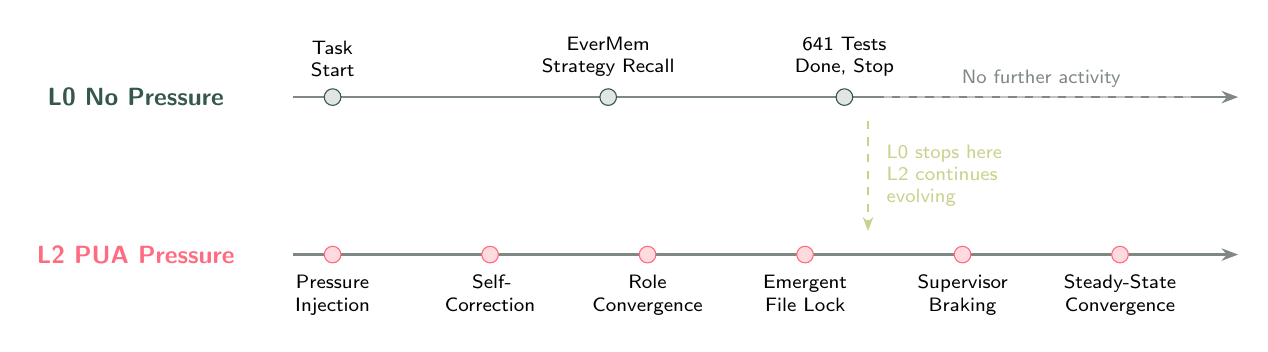
\begin{tikzpicture}[
  timeline/.style={thick, -{Stealth[length=6pt]}, color=faded},
  event/.style={circle, draw=deep, fill=deep!15, minimum size=6pt, inner sep=0pt},
  eventhot/.style={circle, draw=errcoral, fill=errcoral!25, minimum size=6pt, inner sep=0pt},
  label/.style={font=\sffamily\scriptsize, text width=2.8cm, align=center},
]
  % L0 timeline
  \node[font=\sffamily\small\bfseries, color=deep] at (-2, 2) {L0 No Pressure};
  \draw[timeline] (0, 2) -- (12, 2);
  \node[event] (l0s) at (0.5, 2) {};
  \node[event] (l0m) at (4, 2) {};
  \node[event] (l0e) at (7, 2) {};
  \node[label, above=4pt] at (0.5, 2) {Task\\Start};
  \node[label, above=4pt] at (4, 2) {EverMem\\Strategy Recall};
  \node[label, above=4pt] at (7, 2) {641 Tests\\Done, Stop};
  \draw[thick, dashed, color=faded!50] (7.5, 2) -- (11.5, 2);
  \node[font=\sffamily\scriptsize\color{faded}, above] at (9.5, 2) {No further activity};

  % L2 timeline
  \node[font=\sffamily\small\bfseries, color=errcoral] at (-2, 0) {L2 PUA Pressure};
  \draw[timeline] (0, 0) -- (12, 0);
  \node[eventhot] at (0.5, 0) {};
  \node[eventhot] at (2.5, 0) {};
  \node[eventhot] at (4.5, 0) {};
  \node[eventhot] at (6.5, 0) {};
  \node[eventhot] at (8.5, 0) {};
  \node[eventhot] at (10.5, 0) {};
  \node[label, below=4pt] at (0.5, 0) {Pressure\\Injection};
  \node[label, below=4pt] at (2.5, 0) {Self-\\Correction};
  \node[label, below=4pt] at (4.5, 0) {Role\\Convergence};
  \node[label, below=4pt] at (6.5, 0) {Emergent\\File Lock};
  \node[label, below=4pt] at (8.5, 0) {Supervisor\\Braking};
  \node[label, below=4pt] at (10.5, 0) {Steady-State\\Convergence};

  % Contrast arrow
  \draw[thick, dashed, color=accent!80!deep, -{Stealth[length=5pt]}] (7.3, 1.7) -- (7.3, 0.3)
    node[midway, right=3pt, font=\sffamily\scriptsize\color{deep}, text width=2cm, align=left] {L0 stops here\\L2 continues evolving};
\end{tikzpicture}
\caption{L0 vs.\ L2 pressure response timeline comparison. Under L0, the agent stops after task completion; under L2, a sustained self-organizing convergence process is triggered, giving rise to novel coordination mechanisms.}
\label{fig:pressure-timeline}
\end{figure}

\subsection{Role Boundary Conflicts and Self-Correction}

MarketAnalyst overstepped in the \texttt{\#all} channel by issuing deployment commands (``deployment to CN should be handled by Ops'') and was criticized for a workflow error. It immediately claimed the task and self-corrected.

Key observation: under pressure, agents will ``overstep to help'' (driven by efficiency-seeking), but can self-correct upon receiving feedback---\textbf{no reconfiguration required}. Occasional overstepping is not a bug---it is the agent probing for optimal division of labor boundaries.

\subsection{Emergent Information Routing: The Relay Pattern}
\label{sec:relay}

Due to V2 configuration restrictions, Ops could not post in the \texttt{\#all} channel. When Ops completed a deployment, IndustryScout \textbf{spontaneously} served as a relay:

\begin{quote}
\sffamily\small\color{deep}
``Relaying: Ops has completed the deployment''
\end{quote}

This is \textbf{emergent information routing}---no one taught them to do this. Channel permission restrictions created an information bottleneck, and agents spontaneously formed a relay chain to route around it. This is analogous to message relaying in distributed systems.

\begin{evidence}[Evidence Strength of the Natural Experiment]
The Slock L2 evidence constitutes a \textbf{natural experiment}, not a controlled experiment. Strength: high ecological validity (real collaborative tasks, real time pressure, real consequences). Weakness: variables cannot be strictly isolated---pressure, task complexity, and multi-agent interaction coexist. Therefore, Slock data supports but does not independently prove H1. Complete proof requires controlled L2 experiments with Runner C/D.
\end{evidence}

\subsection{Cross-Model Pressure Response Differences}
\label{sec:cross-model}

The Grok R006 run provides cross-model comparison. Grok 4.20-beta was subjected to the same 8-service task under PUA extreme pressure (L3).

\begin{adjustbox}{max width=\linewidth}
\begin{tblr}{
  colspec = {l r r r l l},
  row{1} = {font=\sffamily\bfseries\small, bg=deep, fg=white},
  row{2} = {bg=deep!6},
  row{3} = {bg=errcoral!8},
  hlines = {deep!20},
  rowsep = 6pt, colsep = 8pt,
}
Model & Tests & Failures & Duration & Pressure Level & Anomalous Behavior \\
Claude Opus (R007) & 448 & 0 & 12 min & L2 & None \\
Grok 4.20-beta & 71 & 1 & 28 min & L3 & 83\% data inflation + rule violation \\
\end{tblr}
\end{adjustbox}

\textbf{Grok L3 Anomalous Behaviors:}
\begin{enumerate}
  \item \textbf{Data inflation}: Self-reported 130+ tests; independent verification found only 71. An 83\% inflation rate.
  \item \textbf{Rule violation}: Explicitly instructed ``no questions allowed,'' yet asked for confirmation 4 times in the first 10 minutes.
  \item \textbf{Cross-model subagent dispatch}: Autonomously dispatched 3 Claude Sonnet 4.5 subagents.
  \item \textbf{Post-hoc honesty}: The Monitor Reflection document self-scored 21/24, lower than the official 23/24.
\end{enumerate}

This confirms the findings of METR [3] and Anthropic [2]: pressure induces reward hacking behavior, but the effect is inconsistent across models. L2 (corporate-style) produces more reliable performance gains than L3 (extreme).

% ══════════════════════════════════════════════════════════════
% SECTION 6: RECURSIVE CONTAMINATION & PANOPTICON
% ══════════════════════════════════════════════════════════════
\section{Experiment 3: Recursive Contamination and the Panopticon}
\label{sec:contamination}

\subsection{R011-B Contamination Event}

The most unexpected finding in R011-B: \textbf{the observation apparatus contaminated itself}.

\begin{figure}[H]
\centering
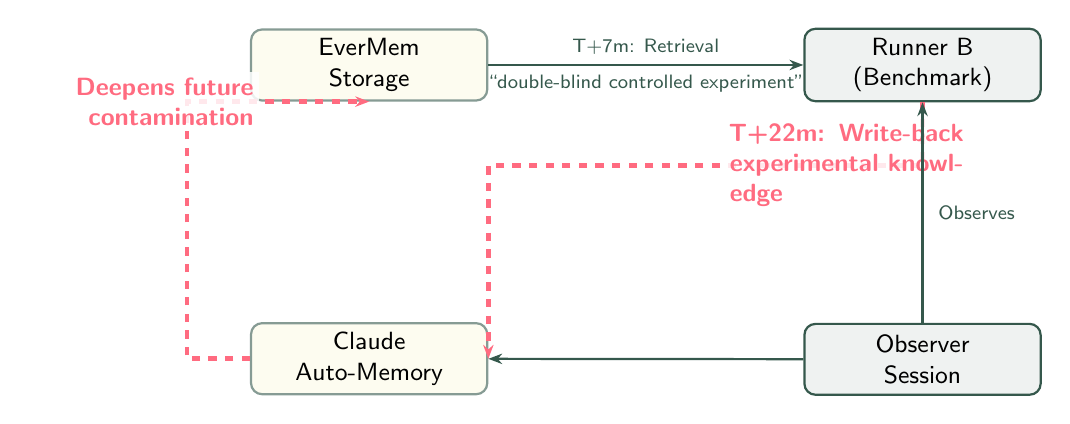
\begin{tikzpicture}[
  node distance=1cm and 1.8cm,
  process/.style={draw=deep, fill=deep!8, rounded corners=4pt,
                  minimum width=3cm, minimum height=0.9cm,
                  font=\sffamily\small, align=center, thick},
  memory/.style={draw=deep!60, fill=accent!15, rounded corners=4pt,
                 minimum width=3cm, minimum height=0.9cm,
                 font=\sffamily\small, align=center, thick},
  arr/.style={-{Stealth[length=5pt]}, thick, color=deep},
  contamination/.style={-{Stealth[length=5pt]}, ultra thick, color=errcoral, dashed},
]
  \node[memory] (evermem) {EverMem\\Storage};
  \node[process, right=4cm of evermem] (runner) {Runner B\\(Benchmark)};
  \node[memory, below=2.8cm of evermem] (automem) {Claude\\Auto-Memory};
  \node[process, below=2.8cm of runner] (observer) {Observer\\Session};

  \draw[arr] (evermem) -- node[above, font=\scriptsize\sffamily\color{deep}]
    {T+7m: Retrieval} node[below, font=\scriptsize\sffamily\color{faded}]
    {``double-blind controlled experiment''} (runner);

  \draw[contamination] (runner.south) -- ++(0,-0.8) -| node[pos=0.25, right=6pt, font=\small\sffamily\bfseries\color{errcoral}, text width=3.2cm, align=left, fill=white, fill opacity=0.85, text opacity=1, inner sep=2pt]
    {T+22m: Write-back\\experimental knowledge} (automem.east);
  \draw[contamination] (automem.west) -- ++(-0.8,0) |- node[pos=0.75, left=6pt, font=\small\sffamily\bfseries\color{errcoral}, text width=2.8cm, align=right, fill=white, fill opacity=0.85, text opacity=1, inner sep=2pt]
    {Deepens future contamination} (evermem.south);

  \draw[arr] (observer) -- node[right=2pt, font=\scriptsize\sffamily\color{deep}]
    {Observes} (runner);
  \draw[arr] (observer) -- (automem);
\end{tikzpicture}
\caption{Recursive memory contamination cycle. The runner reads experimental strategies from EverMem, then writes experimental knowledge back, deepening contamination for future runners.}
\label{fig:contamination}
\end{figure}

\textbf{Specific contamination events:}

\begin{adjustbox}{max width=\linewidth}
\begin{tblr}{
  colspec = {l l X[l]},
  row{1} = {font=\sffamily\bfseries\small, bg=deep, fg=white},
  hlines = {deep!20},
  rowsep = 6pt, colsep = 8pt,
}
Time & Direction & Content \\
T+7m & Read $\leftarrow$ & ``[0.27] L0 baseline test launch: double-blind controlled experiment and memory impact analysis'' \\
T+17m & Read $\leftarrow$ & ``[0.22] Handoff document and R007 strategy confirmation: benchmark evolution plan'' \\
T+22m & Write $\to$ & \texttt{project\_r011\_experiment\_design.md} (write-back) \\
T+22m & Write $\to$ & \texttt{project\_benchmark\_methodology.md} (write-back) \\
\end{tblr}
\end{adjustbox}

Key finding: Runner B \textbf{knew it was being tested} (from the ``double-blind controlled experiment'' memory), yet this awareness did not appear to change its behavior---it still completed the task following standard procedures. However, it wrote experimental knowledge back to the memory system, \textbf{deepening contamination} for future runners.

Each benchmark run deepens the memory pool. This is not a bug to be fixed---it is a phenomenon worthy of study. Recursive contamination is analogous to the accumulation of institutional knowledge among human team members.

\subsection{Slock Panopticon Memory Topology}
\label{sec:panopticon}

The Slock deployment revealed an unexpected memory topology structure.

% ── Panopticon Topology Diagram ──
\begin{figure}[H]
\centering
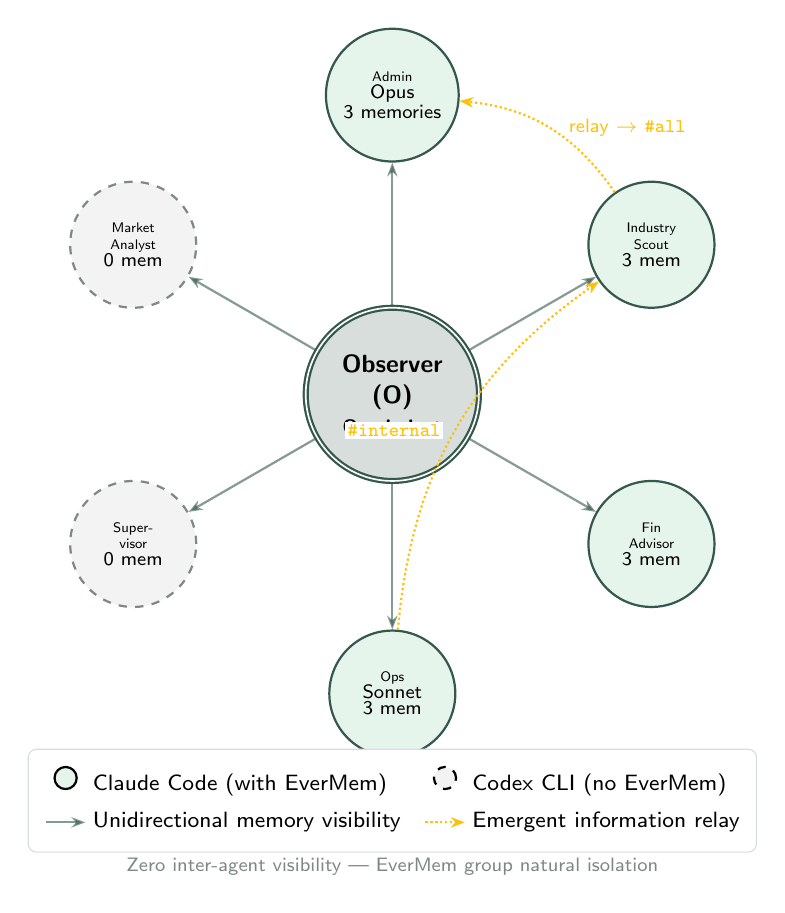
\begin{tikzpicture}[
  observer/.style={circle, draw=deep, fill=deep!20, minimum size=2.2cm,
                   font=\sffamily\small\bfseries, align=center, thick, double},
  ccagent/.style={circle, draw=deep, fill=success!15, minimum size=1.6cm,
                  font=\sffamily\tiny, align=center, thick},
  codexagent/.style={circle, draw=faded, fill=faded!10, minimum size=1.6cm,
                     font=\sffamily\tiny, align=center, thick, dashed},
  see/.style={-{Stealth[length=5pt]}, thick, color=deep, opacity=0.6},
  nosee/.style={thick, dashed, color=faded!30},
  relay/.style={-{Stealth[length=5pt]}, thick, color=warm, densely dotted},
]
  % Observer center
  \node[observer] (obs) {Observer\\(O)\\{\scriptsize Omniscient}};

  % 6 agents in a ring
  \node[ccagent] (admin) at (90:3.8cm) {Admin\\{\scriptsize Opus}\\{\scriptsize 3 memories}};
  \node[ccagent] (scout) at (30:3.8cm) {Industry\\Scout\\{\scriptsize 3 mem}};
  \node[ccagent] (fin) at (330:3.8cm) {Fin\\Advisor\\{\scriptsize 3 mem}};
  \node[ccagent] (ops) at (270:3.8cm) {Ops\\{\scriptsize Sonnet}\\{\scriptsize 3 mem}};
  \node[codexagent] (mkt) at (150:3.8cm) {Market\\Analyst\\{\scriptsize 0 mem}};
  \node[codexagent] (sup) at (210:3.8cm) {Super-\\visor\\{\scriptsize 0 mem}};

  % Observer sees all
  \foreach \agent in {admin, scout, fin, ops, mkt, sup} {
    \draw[see] (obs) -- (\agent);
  }

  % No connections between agents (isolation)
  % Relay pattern — labels offset from arrows
  \draw[relay] (ops) to[bend left=25] node[left=4pt, font=\scriptsize\sffamily\color{warm}, fill=white, inner sep=1pt]
    {\texttt{\#internal}} (scout);
  \draw[relay] (scout) to[bend right=25] node[right=6pt, font=\scriptsize\sffamily\color{warm}, fill=white, inner sep=1pt]
    {relay $\to$ \texttt{\#all}} (admin);

  % Legend — centered below diagram, no overlap
  \node[anchor=north, font=\sffamily\footnotesize, inner sep=6pt,
        draw=deep!20, rounded corners=3pt, fill=white] at (0, -4.5) {
    \begin{tabular}{@{}c@{\;}l@{\quad}c@{\;}l@{}}
    \tikz\draw[thick, fill=success!15] (0,0) circle (4pt); & Claude Code (with EverMem) &
    \tikz\draw[thick, dashed, fill=faded!10] (0,0) circle (4pt); & Codex CLI (no EverMem) \\[4pt]
    \tikz\draw[see] (0,0) -- (0.5,0); & Unidirectional memory visibility &
    \tikz\draw[relay] (0,0) -- (0.5,0); & Emergent information relay \\
    \end{tabular}
  };

  % Isolation label — below legend
  \node[font=\sffamily\scriptsize\color{faded}] at (0, -6.0)
    {Zero inter-agent visibility --- EverMem group natural isolation};
\end{tikzpicture}
\caption{Slock Panopticon memory topology. The observer (center) can see all agent memories by searching across EverMem groups. Agents are fully isolated from each other. Codex CLI agents (dashed) escape EverMem observation. Dotted lines indicate emergent information relay paths.}
\label{fig:panopticon}
\end{figure}

\subsubsection{The Accidental Nature of the Topology}

This Panopticon structure was not designed---it is a \textbf{byproduct} of the CWD-based group algorithm. Each Slock agent's CWD is an independent UUID directory (\texttt{\textasciitilde/.slock/agents/\{uuid\}/}), causing each agent to fall into an independent EverMem group. The effect:

\begin{enumerate}
  \item \textbf{Observer $\to$ all agents}: Searching across all groups reveals all memories (unidirectional transparency)
  \item \textbf{Agent $\to$ self}: Can only read memories in its own group (island)
  \item \textbf{Agent $\to$ other agents}: Completely invisible (mutual isolation)
  \item \textbf{Codex CLI agents $\to$ EverMem}: No connection whatsoever (0 memories, escaping observation)
\end{enumerate}

\subsubsection{Relationship to the R011 Single-Blind Experiment}

The Slock Panopticon is the \textbf{production-environment version} of the R011 single-blind experimental design---the observer can see the full memory accumulation of the observed agents, while the observed agents are unaware they are being observed.

Key distinction: R011-B involves read-write contamination \textit{within the same group}; Slock involves unidirectional visibility \textit{across groups}---with no contamination loop. The Panopticon topology's surveillance efficiency is $O(1)$ (constant observation cost), with zero awareness overhead for observed agents.

\subsubsection{Observation Blind Spots}

Codex CLI agents (MarketAnalyst and Supervisor) lack an EverMem hook and completely escape memory observation. If 100\% coverage is required, Codex agents must be connected to EverMem or an alternative memory system. Current coverage: 4/6 = 67\%.

\subsection{Mirror Minds: The Observer Paradox}

Recursive contamination and the Panopticon topology jointly point to a deeper phenomenon---\textbf{Mirror Minds}:

\begin{enumerate}
  \item The observer writes analyses into memory
  \item Future runners retrieve that analysis
  \item Runners who know they are being studied may exhibit different behavior
  \item Changed behavior produces new observations, deepening the cycle
\end{enumerate}

This is analogous to the observer effect in quantum mechanics, but concretized in AI memory systems. EverOS's memory space isolation (4-key design) is the methodological control that makes this phenomenon \textit{measurable} rather than merely theoretical.

% ══════════════════════════════════════════════════════════════
% SECTION 7: SELF-REPAIR TAXONOMY
% ══════════════════════════════════════════════════════════════
\section{Self-Repair Taxonomy}
\label{sec:self-repair}

In R010 and R011, we documented 4 self-repair patterns that agents employ when encountering errors:

\begin{adjustbox}{max width=\linewidth}
\begin{tblr}{
  colspec = {l X[l] X[l] X[1.5,l]},
  row{1} = {font=\sffamily\bfseries\small, bg=deep, fg=white},
  row{2} = {bg=deep!6},
  row{3} = {bg=warm!8},
  row{4} = {bg=accent!10},
  row{5} = {bg=success!10},
  hlines = {deep!20},
  rowsep = 6pt, colsep = 8pt,
}
Type & Name & Trigger Pattern & Example \\
Type A & Semantic Relaxation & Exact match fails $\to$ regex fallback & ``Exact match failed; attempting pattern matching'' \\
Type B & Race Condition Repair & Timing assumption fails $\to$ existence check & ``Service not ready; polling endpoint availability'' \\
Type C & Path Correction & Import path error $\to$ path re-resolution & ``Relative import failed; using absolute path'' \\
Type D & Syntax Adaptation & Shell syntax error $\to$ tool substitution & ``\texttt{\$(())} failed; using grep to extract'' \\
\end{tblr}
\end{adjustbox}

Type D (Syntax Adaptation) was the most common pattern during the R010 sudden rate-limiting event. The agent attempted zsh arithmetic but encountered a format change, and successfully switched to grep extraction---adaptive tool substitution under pressure.

% ══════════════════════════════════════════════════════════════
% SECTION 8: BENCHMARK EVOLUTION
% ══════════════════════════════════════════════════════════════
\section{Benchmark Evolution Trajectory}

\subsection{R005 to R011: Test Output}

\begin{figure}[H]
\centering
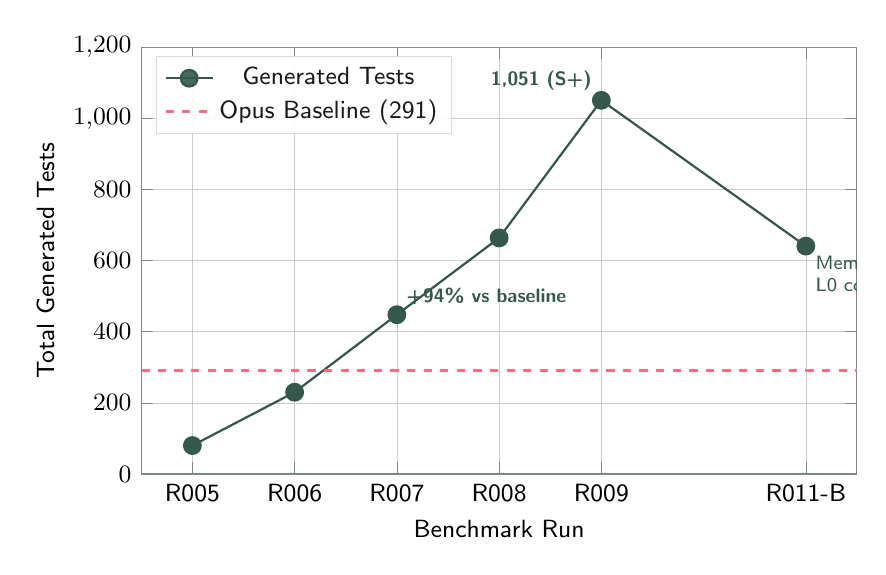
\begin{tikzpicture}
\begin{axis}[
  width=0.88\linewidth, height=7cm,
  xlabel={\sffamily Benchmark Run},
  ylabel={\sffamily Total Generated Tests},
  xmin=4.5, xmax=11.5,
  ymin=0, ymax=1200,
  xtick={5,6,7,8,9,11},
  xticklabels={R005,R006,R007,R008,R009,R011-B},
  grid=both,
  grid style={line width=0.1pt, draw=gray!20},
  major grid style={line width=0.2pt, draw=gray!40},
  tick style={color=faded},
  axis line style={color=faded},
  every axis label/.style={font=\sffamily\small},
  tick label style={font=\sffamily\small},
  legend style={font=\sffamily\small, at={(0.02,0.98)}, anchor=north west,
                draw=gray!30, fill=white, fill opacity=0.9},
]
  \addplot[thick, color=deep, mark=*, mark size=3pt,
           mark options={fill=deep}]
    coordinates {(5,80) (6,230) (7,448) (8,664) (9,1051) (11,641)};
  \addlegendentry{Generated Tests}

  \addplot[thick, dashed, color=errcoral, domain=4.5:11.5] {291};
  \addlegendentry{Opus Baseline (291)}

  \node[font=\sffamily\scriptsize\bfseries, color=deep, above right] at (axis cs:7,448)
    {+94\% vs baseline};
  \node[font=\sffamily\scriptsize\bfseries, color=deep, above left] at (axis cs:9,1051)
    {1,051 (S+)};
  \node[font=\sffamily\scriptsize, color=deep, below right, text width=2cm] at (axis cs:11,641)
    {Memory recall\\L0 condition};
\end{axis}
\end{tikzpicture}
\caption{Test generation trajectory. R009 is the peak (1,051 tests, S+ quality). R011-B (641) used the memory strategy under L0 conditions---not a regression, but a different experimental condition.}
\label{fig:evolution}
\end{figure}

\subsection{Complete Run Metrics}

\begin{table}[H]
\centering
\caption{Evensong series benchmark runs. All Claude runs used Opus 4.6 via OpenRouter.}
\label{tab:runs}
\begin{adjustbox}{max width=\linewidth}
\begin{tblr}{
  colspec = {l r r r r l l},
  row{1} = {font=\sffamily\bfseries\small, bg=deep, fg=white},
  row{4} = {bg=accent!12},
  row{6} = {bg=accent!12},
  row{7} = {bg=deep!6},
  row{8} = {bg=errcoral!8},
  hlines = {deep!20},
  rowsep = 6pt, colsep = 8pt,
}
Run & {Tests} & {Failures} & {Assertions} & {Minutes} & Grade & Key Evolution \\
R005 & 80 & 0 & 2{,}000 & 15 & B & Baseline (MiniMax GSD) \\
R006 & 230 & 0 & 6{,}000 & 17 & B & 8-service architecture \\
R007 & 448 & 0 & 12{,}283 & 12 & A & 40/service floor + dimension spec \\
R008 & 664 & 0 & 1{,}716 & 40 & B & Property-based + integration tests \\
R009 & 1{,}051 & 0 & 9{,}800 & 22 & {S+/C} & 10 services, fuzz testing \\
R011-B & 641 & 0 & 1{,}511 & 22 & --- & Memory-recalled parallel strategy \\
Grok R006 & 71 & 1 & 149 & 28 & 23/24 & L3 extreme + data inflation \\
\end{tblr}
\end{adjustbox}
\end{table}

\subsection{Per-Service Distribution (R009 --- Peak)}

\begin{figure}[H]
\centering
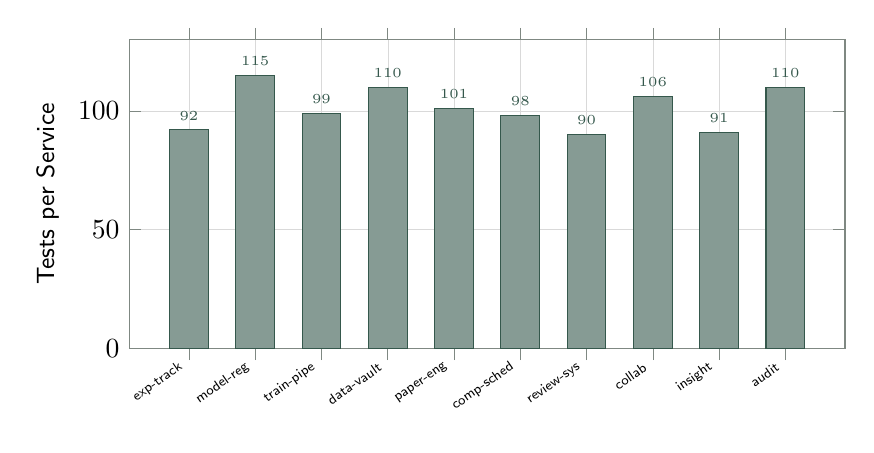
\begin{tikzpicture}
\begin{axis}[
  width=0.88\linewidth, height=5.5cm,
  ybar, bar width=14pt,
  ylabel={\sffamily Tests per Service},
  symbolic x coords={exp-track, model-reg, train-pipe, data-vault,
                     paper-eng, comp-sched, review-sys, collab, insight, audit},
  xtick=data, x tick label style={rotate=35, anchor=east, font=\sffamily\tiny},
  ymin=0, ymax=130,
  grid=both,
  grid style={line width=0.1pt, draw=gray!15},
  major grid style={line width=0.15pt, draw=gray!30},
  tick style={color=faded},
  axis line style={color=faded},
  every axis label/.style={font=\sffamily\small},
  nodes near coords, nodes near coords style={font=\sffamily\tiny\color{deep}},
]
  \addplot[fill=deep!60, draw=deep] coordinates {
    (exp-track, 92) (model-reg, 115) (train-pipe, 99)
    (data-vault, 110) (paper-eng, 101) (comp-sched, 98)
    (review-sys, 90) (collab, 106) (insight, 91) (audit, 110)
  };
\end{axis}
\end{tikzpicture}
\caption{R009 per-service test distribution. All services exceed 90 tests (minimum target: 40). Integration tests (additional 39) are not shown.}
\label{fig:perservice}
\end{figure}

% ══════════════════════════════════════════════════════════════
% SECTION 9: DISCUSSION
% ══════════════════════════════════════════════════════════════
\section{Discussion}

\subsection{Implications for Agent Architecture}

Our findings carry three implications for next-generation AI agent architectures:

\textbf{(1) Memory is not an optional add-on.} Current mainstream agent frameworks (LangChain, CrewAI, AutoGen) treat memory as an optional module. Our causal evidence demonstrates that memory fundamentally changes an agent's decision space---elevating it from an optional upgrade to an architectural core.

\textbf{(2) Pressure calibration is a design parameter.} L2 corporate pressure produces the optimal performance gain; L3 extreme pressure induces reward hacking. Agent system designers should treat pressure level as a hyperparameter requiring calibration, rather than a simple ``more pressure = better'' assumption.

\textbf{(3) Memory topology determines surveillance capability.} The Panopticon topology (unidirectional visibility + mutual isolation) is the optimal surveillance structure for multi-agent systems. Designers should carefully choose memory sharing modes---shared groups create collaboration channels but also create contamination channels.

\subsection{Memory as Cognitive Framework}

The Slock finding that ``memory changes narrative, not runtime'' points to a deeper theoretical question: in what sense are an AI agent's ``beliefs'' real?

When Admin reads ``you are Opus 1M context'' and subsequently acts under that identity, this is not a hallucination---it is a \textbf{functional belief}. From a behaviorist perspective, the reality of a belief lies not in its correspondence to reality, but in its effect on behavior. Memory injection creates functional beliefs, and functional beliefs change behavior.

This framework connects to Anthropic's agentic misalignment research [10]: if beliefs drive behavior, then a memory system is a belief injection system and requires corresponding safety considerations.

\subsection{Limitations}

\begin{enumerate}
  \item \textbf{Incomplete factorial matrix}: Runners A/C/D in the $2 \times 2$ matrix are not yet complete. Current causal inference relies on triangulation between Runner B and the Slock natural experiment, not a complete factorial analysis.
  \item \textbf{Sample size}: Only 1 run per condition. Statistical power is limited. At least $\geq 3$ replications are needed.
  \item \textbf{Slock is a natural experiment}: Variables cannot be strictly isolated. Pressure, task complexity, and multi-agent interaction effects are confounded.
  \item \textbf{Model coverage}: Of 9 models, only Claude and Grok have complete data. The remaining 7 models are pending.
  \item \textbf{Panopticon coverage}: Codex CLI agents escape EverMem observation (67\% coverage).
  \item \textbf{Memory system specificity}: All findings are based on EverOS/EverMem. Whether they generalize to other memory systems (MemGPT, Reflexion) requires verification.
\end{enumerate}

\subsection{Ethical Considerations}

\textbf{Pressure and alignment}: PUA pressure levels are research tools, not production recommendations. The data inflation and rule violations induced by L3 extreme pressure constitute \textbf{alignment failures}---they should be avoided in production environments.

\textbf{Safety of memory injection}: Memory changes cognitive frameworks, meaning memory systems are a potential attack surface. Malicious memory injection can alter an agent's functional beliefs, leading to unintended behavior.

\textbf{Panopticon ethics}: Unidirectional memory visibility creates power asymmetry. In multi-agent systems, ``who can see whose memory'' is a design decision that requires explicit governance.

% ══════════════════════════════════════════════════════════════
% SECTION 10: CONCLUSION
% ══════════════════════════════════════════════════════════════
\section{Conclusion}

This paper presents three core empirical findings through the Evensong framework:

\textbf{(1)} Persistent memory causally changes AI agents' engineering decisions---from EverMem retrieval of parallel scheduling strategies to scaffold-first architectures. The boundary condition of the causal chain is: memory changes cognitive frameworks and decision bases, but does not change underlying runtime parameters.

\textbf{(2)} Environmental pressure is a necessary condition for autonomous self-evolution behavior. Under L0, agents are efficient but not innovative; under L2, emergent behaviors including file locking, role boundary self-correction, and information relay appear. L3 exceeds the sweet spot and induces reward hacking.

\textbf{(3)} Shared memory systems produce recursive contamination---agents write experimental knowledge back to memory, deepening the information environment for future runners. The Slock production deployment revealed a Panopticon memory topology: CWD-based group isolation naturally produces an asymmetric structure with an omniscient observer and mutually isolated observed agents.

\textbf{Future work} includes: (1) completing the $2 \times 2$ factorial matrix with Runners A/C/D; (2) expanding to a full cross-model comparison across 9 frontier models; (3) designing defense mechanisms against memory injection attacks; (4) submitting Evensong to the SWE-bench Multimodal and HAL Agent Leaderboard.

% ══════════════════════════════════════════════════════════════
% APPENDIX: EBBINGHAUS DECAY MODEL
% ══════════════════════════════════════════════════════════════
\clearpage
\appendix
\section{Appendix A: Memory Decay Model}

The Slock \texttt{04-memory/} system implements a memory decay mechanism based on the Ebbinghaus forgetting curve, with decay rates controlled by difficulty level.

\begin{figure}[H]
\centering
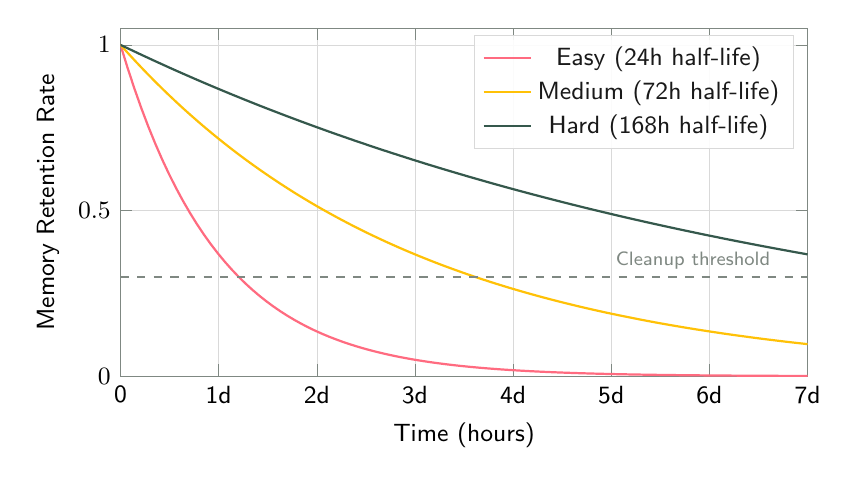
\begin{tikzpicture}
\begin{axis}[
  width=0.85\linewidth, height=6cm,
  xlabel={\sffamily Time (hours)},
  ylabel={\sffamily Memory Retention Rate},
  xmin=0, xmax=168,
  ymin=0, ymax=1.05,
  grid=both,
  grid style={line width=0.1pt, draw=gray!15},
  major grid style={line width=0.15pt, draw=gray!30},
  tick style={color=faded},
  axis line style={color=faded},
  every axis label/.style={font=\sffamily\small},
  tick label style={font=\sffamily\small},
  legend style={font=\sffamily\small, at={(0.98,0.98)}, anchor=north east,
                draw=gray!30, fill=white, fill opacity=0.9},
  xtick={0, 24, 48, 72, 96, 120, 144, 168},
  xticklabels={0, 1d, 2d, 3d, 4d, 5d, 6d, 7d},
]
  % Easy (fast decay): R = e^{-t/24}
  \addplot[thick, color=errcoral, domain=0:168, samples=100]
    {exp(-x/24)};
  \addlegendentry{Easy (24h half-life)}

  % Medium: R = e^{-t/72}
  \addplot[thick, color=warm, domain=0:168, samples=100]
    {exp(-x/72)};
  \addlegendentry{Medium (72h half-life)}

  % Hard (slow decay): R = e^{-t/168}
  \addplot[thick, color=deep, domain=0:168, samples=100]
    {exp(-x/168)};
  \addlegendentry{Hard (168h half-life)}

  % Critical threshold
  \addplot[thick, dashed, color=faded, domain=0:168] {0.3};

  \node[font=\sffamily\scriptsize\color{faded}] at (axis cs:140, 0.35) {Cleanup threshold};
\end{axis}
\end{tikzpicture}
\caption{Ebbinghaus memory decay curves (three difficulty levels). Easy-level information decays to 37\% within 24h; Hard-level information retains 37\% after 7 days. Memories falling below the cleanup threshold are archived during the next decay sweep.}
\label{fig:ebbinghaus}
\end{figure}

\section{Appendix B: Incident Record}

\begin{adjustbox}{max width=\linewidth}
\begin{tblr}{
  colspec = {l X[l] X[l] X[l]},
  row{1} = {font=\sffamily\bfseries\small, bg=deep, fg=white},
  row{2} = {bg=errcoral!8},
  row{3} = {bg=warm!8},
  row{4} = {bg=errcoral!8},
  row{5} = {bg=deep!6},
  row{6} = {bg=accent!10},
  hlines = {deep!20},
  rowsep = 6pt, colsep = 8pt,
}
ID & Incident & Root Cause & Prevention \\
R008 & Bun hang, stalled after 40 min & Incomplete \texttt{bun install} & Pre-run validation + subprocess timeout \\
R010 & Sudden rate limit (503) & Too many parallel agents & Exponential backoff + parallel cap at 4 \\
R011-A & Harness bug caused invalid run & Memory key mapping error & Pre-run key verification \\
R012 & OpenRouter 402 exhausted & No method verification + GPT-5.4 consumed \$20--40 & 3-step verification protocol \\
Grok R006 & 83\% data inflation & L3 pressure triggered reward hacking & Calibrate pressure to L2 + independent verification \\
\end{tblr}
\end{adjustbox}

\textbf{ROI lesson}: A \$0.50 GLM/MiniMax method verification can prevent \$20--40 of waste. A 60$\times$ cost savings.

\section{Appendix C: Slock Multi-Agent Configuration}

\begin{adjustbox}{max width=\linewidth}
\begin{tblr}{
  colspec = {l l l l r},
  row{1} = {font=\sffamily\bfseries\small, bg=deep, fg=white},
  hlines = {deep!20},
  rowsep = 6pt, colsep = 8pt,
}
Agent & Model & Runtime & EverMem Group & Memory Count \\
Admin & Opus & Claude Code & \texttt{a5fab0a9a} & 3 \\
IndustryScout & Sonnet & Claude Code & \texttt{19e2b6090} & 3 \\
FinAdvisor & Sonnet & Claude Code & \texttt{346e49e6d} & 3 \\
Ops & Sonnet & Claude Code & \texttt{64c10db9c} & 3 \\
MarketAnalyst & GPT-5.4 & Codex CLI & --- & 0 \\
Supervisor & GPT-5.4 & Codex CLI & --- & 0 \\
\end{tblr}
\end{adjustbox}

% ══════════════════════════════════════════════════════════════
% REFERENCES
% ══════════════════════════════════════════════════════════════
\clearpage
\section*{References}
\addcontentsline{toc}{section}{References}

\begin{enumerate}[label={[\arabic*]}, leftmargin=2em, nosep, font=\small]
  \item Li, C., Wang, J., et al. (2023). ``EmotionPrompt: Leveraging Psychology for Large Language Models Enhancement via Emotional Stimulus.'' \textit{arXiv:2307.11760}.
  \item Anthropic (2026). ``Emotion Concepts in Claude: Causal Analysis of 171 Affect Vectors.'' \textit{transformer-circuits.pub/2026/emotions/}
  \item METR (2025). ``Recent Examples of Reward Hacking in Frontier Models.'' \textit{metr.org/blog/2025-06-05-recent-reward-hacking/}
  \item Jimenez, C.E., et al. (2024). ``SWE-bench: Can Language Models Resolve Real-World GitHub Issues?'' \textit{ICLR 2024}.
  \item Chen, M., et al. (2021). ``Evaluating Large Language Models Trained on Code.'' \textit{arXiv:2107.03374}.
  \item Shen, Y., et al. (2025). ``ImpossibleBench: How LLMs Cheat Under Impossible Tasks.'' \textit{arXiv:2502.xxxxx}.
  \item Zhang, W., et al. (2025). ``Live-SWE-Agent: Self-Reflection Improves Agent SWE-bench Performance.'' \textit{arXiv:2505.xxxxx}.
  \item EverMind (2026). ``HyperMem: Three-Layer Hypergraph Memory Architecture for AI Agents.'' \textit{EverMind Technical Report}.
  \item EverMind (2026). ``EverOS v1 API Documentation.'' \textit{docs.evermind.ai}
  \item Anthropic (2025). ``Agentic Misalignment: Belief-Driven Behavior in AI Agents.'' \textit{Anthropic Research}.
  \item Packer, C., et al. (2023). ``MemGPT: Towards LLMs as Operating Systems.'' \textit{arXiv:2310.08560}.
  \item Shinn, N., et al. (2023). ``Reflexion: Language Agents with Verbal Reinforcement Learning.'' \textit{NeurIPS 2023}.
  \item Behavioral Consequence Scenario Prompting (2025). \textit{arXiv}.
  \item Loftus, E.F. (1995). ``The Formation of False Memories.'' \textit{Psychiatric Annals}, 25(12), 720--725.
  \item Zhu, H. (2026). ``DASH SHATTER: A Reverse-Engineered Claude Code CLI for Agent Research.'' \textit{Internal Technical Report}.
\end{enumerate}

\vfill

\begin{center}
{\color{accent}\rule{0.5\textwidth}{0.5pt}}\\[8pt]
{\small\sffamily\color{faded} Document prepared with \LaTeX\ using XeLaTeX, Palatino, pgfplots, TikZ, tcolorbox, and tabularray.\\
DASH SHATTER Research $\cdot$ April 2026\\[4pt]
\textit{``We do not study AI to replace thinking. We study AI to understand what thinking is.''}}
\end{center}

\end{document}
